%%%%%%%%%%%%%%%%%%%%%%%%%%%%%%%%%%%%%%%%%%%%%%%%%%%%%%%%%%%%%%%%%%%%%%%%%%%%%%%%
%2345678901234567890123456789012345678901234567890123456789012345678901234567890
%        1         2         3         4         5         6         7         8

\documentclass[letterpaper, 10 pt, conference]{ieeeconf}  % Comment this line out if you need a4paper

%\documentclass[a4paper, 10pt, conference]{ieeeconf}      % Use this line for a4 paper

\IEEEoverridecommandlockouts                              % This command is only needed if 
                                                          % you want to use the \thanks command

\overrideIEEEmargins                                      % Needed to meet printer requirements.

%In case you encounter the following error:
%Error 1010 The PDF file may be corrupt (unable to open PDF file) OR
%Error 1000 An error occurred while parsing a contents stream. Unable to analyze the PDF file.
%This is a known problem with pdfLaTeX conversion filter. The file cannot be opened with acrobat reader
%Please use one of the alternatives below to circumvent this error by uncommenting one or the other
%\pdfobjcompresslevel=0
%\pdfminorversion=4

% See the \addtolength command later in the file to balance the column lengths
% on the last page of the document

% The following packages can be found on http:\\www.ctan.org
%\usepackage{graphics} % for pdf, bitmapped graphics files
%\usepackage{epsfig} % for postscript graphics files
%\usepackage{mathptmx} % assumes new font selection scheme installed
%\usepackage{times} % assumes new font selection scheme installed
%\usepackage{amsmath} % assumes amsmath package installed
%\usepackage{amssymb}  % assumes amsmath package installed

\usepackage[portuguese]{babel}
\usepackage[utf8]{inputenc}
\usepackage[T1]{fontenc}
\usepackage[dvips]{graphicx}
\usepackage{caption}
\usepackage{subcaption}
\usepackage[scale=0.8]{geometry} % Reduce document margins
\usepackage{minted}    
\usepackage{fancyvrb,newverbs,xcolor}
\usepackage{titlesec}
\usepackage{multirow}

\title{\LARGE \bf
Resolução do Lunar Lander com DQN 
}


\author{Andrei Albani, Bruno Daigo Yamamoto e Vinicius José de Menezes Pereira}% % <-this % stops a space

% \thanks{*This work was not supported by any organization}% <-this % stops a space
% \thanks{$^{1}$Albert Author is with Faculty of Electrical Engineering, Mathematics and Computer Science,
%        University of Twente, 7500 AE Enschede, The Netherlands
%        {\tt\small albert.author@papercept.net}}%
% \thanks{$^{2}$Bernard D. Researcheris with the Department of Electrical Engineering, Wright State University,
%        Dayton, OH 45435, USA
%        {\tt\small b.d.researcher@ieee.org}}%
%}


\begin{document}



\maketitle
\thispagestyle{empty}
\pagestyle{empty}


%%%%%%%%%%%%%%%%%%%%%%%%%%%%%%%%%%%%%%%%%%%%%%%%%%%%%%%%%%%%%%%%%%%%%%%%%%%%%%%%
\begin{abstract}
Resolução do problema \emph{Lunar Lander} do \emph{OpenAI Gym} utilizando redes neurais profundas e aprendizado por reforço. Utilizou-se \emph{reward engineering} para melhorar o aprendizado, mas não foi suficiente para obter resultados satisfatórios. Avaliamos estratégias que tiveram melhor desempenho.


\end{abstract}


%%%%%%%%%%%%%%%%%%%%%%%%%%%%%%%%%%%%%%%%%%%%%%%%%%%%%%%%%%%%%%%%%%%%%%%%%%%%%%%%
\section{Introdução e Motivação}

Em outubro de 2015, o \emph{AlphaGo} tornou-se o primeiro programa de computador a derrotar um jogador profissional do jogo Go nas regras clássicas, sem desvantagem inicial alguma para o jogador humano. O jogo de Go é considerado mais difícil de ser jogado por inteligências aritificias do que outros jogos de tabuleiro, como xadrez ou damas, por possuir um fator de ramificação muitas vezes maior que o desses. Desse modo, o uso de métodos tradicionais de inteligência artificial não é capaz de tornar um programa competitivo a ponto de vencer os melhores jogadores profissionais[1]. A vitória do \emph{AlphaGo}, portanto, foi um marco na história dos métodos de inteligência artificial. A \emph{DeepMind}, desenvolvedora do programa, utilizou no \emph{AlphaGo} o algoritmo de busca \emph{Monte Carlo Tree Search} guiado por uma rede neural profunda. Inicialmente, a rede foi treinada com aprendizado supervisionado, utilizando como base partidas de jogares profissionais, com o chamado \emph{Imitation Learning}, e depois passou por um aprendizado por reforço profundo. Já em outubro de 2017, a \emph{DeepMind} lançou uma nova IA: o \emph{AlphaGo Zero}, o qual foi instruído com as regras básicas do jogo de Go e posto em um processo de aprendizado por reforço no qual jogou consigo mesmo por milhões de partidas. Após um período de treinamento de apenas três dias, o \emph{AlphaGo Zero} venceu 100 de 100 partidas jogadas contra o \emph{AlphaGo} original, demonstrando, com isso, o grande potencial que existe por detrás dos métodos de aprendizado por reforço.

Baseando-nos no grande poder dos algoritmos de Aprendizado de Máquina, em especial o aprendizado por reforço profundo, o qual se mostra muito promissor, como nos mostra a história por detrás do \emph{AlphaGo} decidimos  resolver o problema chamado  \emph{Lunar Lander} disponível pelo framework \emph{OpenAI} utilizando uma rede neural profunda que utiliza aprendizado por reforço, conhecida popularmente por \emph{DQN}.


\section{Apresentação do problema}

O problema do Lunar Lander do \emph{OpenAI} consiste em aterrissar uma nave espacial na superfície de um planeta, no local delimitado por duas bandeiras, como se pode ver na Figura 1:

\begin{figure}[H]
\centering
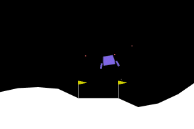
\includegraphics[width=0.3\textwidth]{a.png}
\caption{Apresentação do Lunar Lander}
\label{fig:comparacao}
\end{figure}

O combustível da na nave é teoricamente infinito, podendo ser executadas quatro ações: ligar propulsor esquerdo, ligar o propulsor direito, ligar o propulsor principal ou não fazer nada. O espaço de ação de 4 dimensões é descrito na Tabela 1:

\begin{table}[h]
\caption{Action space: Discrete(4)}
\label{table_example}
\begin{center}
\begin{tabular}{|c|}
\hline
 Do nothing\\
\hline
Fire Left\\
\hline
Fire Main\\
\hline
Fire Right\\
\hline
\end{tabular}
\end{center}
\end{table}

As observações utilizadas no aprendizado por reforço profundo para cada tempo foram 8: as posições x e y, a velocidades em x e y, o ângulo da nave, a velocidade angular e as informações de se cada pé da nave toca a superfície planetária. Isto pode ser visto na Tabela 2:

\\
\begin{center}
TABLE 2: Observation Space
\begin{tabular}
{ |p{2.0cm}||p{1.0cm}|p{1.0cm}|p{1.0cm}|  }
 \hline
 \multicolumn{4}{|c|}{Observation space: (8)} \\
 \hline
 Observation& Type&Min&Max\\
 \hline
 x position & float&-1.5&1.5\\
 y position & float&-1.5&1.5\\
 x velocity & float&-5.0&5.0\\
 y velocity & float&-5.0&5.0\\
 Angle   & float&-3.14&3.14\\
 Ang velocity & float&-5.0&5.0\\
  Left Leg & bool& False&True\\
 Right Leg & bool& False&True\\
 \hline
\end{tabular}
\end{center}
\\
\textfloatsep


No problema, poderiam ter sidos adicionados espaço contínuo, vento e turbulência, mas por simplicidade, decidimos considerar apenas a gravidade no pouso, sem efeitos mais complexos. 

No aprendizado por reforço, o próprio ambiente do \emph{OpenAI} já possuía uma recompensa, chamada em inglês de \emph{reward}, embutida, que penalizava comportamento indesejados como: sair da região de pouso, colidir, utilizar o propulsor(teoricamente deseja-se que o mínimo de combustível seja gasto). Além disso, parabenizava bons comportamentos como: descer e parar, atingir o objetivo. Com a \emph{reward} proposta pela documentação do \emph{OpenAI Gym}, porém, o treinamento da rede neural é lento. Por isso, optamos por adicionar algumas heurísticas na recompensa, assunto melhor abordado na seção \emph{IV.B} e na seção V.

\section{Revisão Teórica}

O algoritmo de \emph{Q-Learning} é uma técnica de aprendizado baseado em valor, ou seja, atualizam a função de valor com base em uma equação, em que a mais utilizada é a equação de Bellman. O \emph{Q-Learning} é um algoritmo \emph{off-policy}, ou seja ele pode atualizar as funções de valor estimado usando ações hipotéticas, aquelas que nunca foram testadas. 

O algoritmo de \emph{Q-Learning} cria uma tabela (matriz) exata para o agente a qual ele observa para maximizar sua recompensa a longo prazo durante seu aprendizado. Esse algoritmo funciona, mas é usado na pratica, apenas para ambientes pequenos e perde seu interesse quando o numero de estados e ações no ambiente aumenta.

Para solucionar esse problema foi criado um novo algoritmo chamado \emph{Deep Q-Network}, que usa uma rede neural profunda para aproximar os valores, tal que essa aproximação não prejudica o aprendizado, desde que a importância relativa seja preservada. 

Ou seja, a principal diferença entre o aprendizado \emph{Q-Learning} e o \emph{Deep Q-Network} é a substituição da \emph{Q Table} do \emph{Q-Learning} por uma rede neural para o aprendizado dos valores de Q. A Figura 2 mostra a comparação dos dois algoritmos.

\begin{figure}[H]
\centering
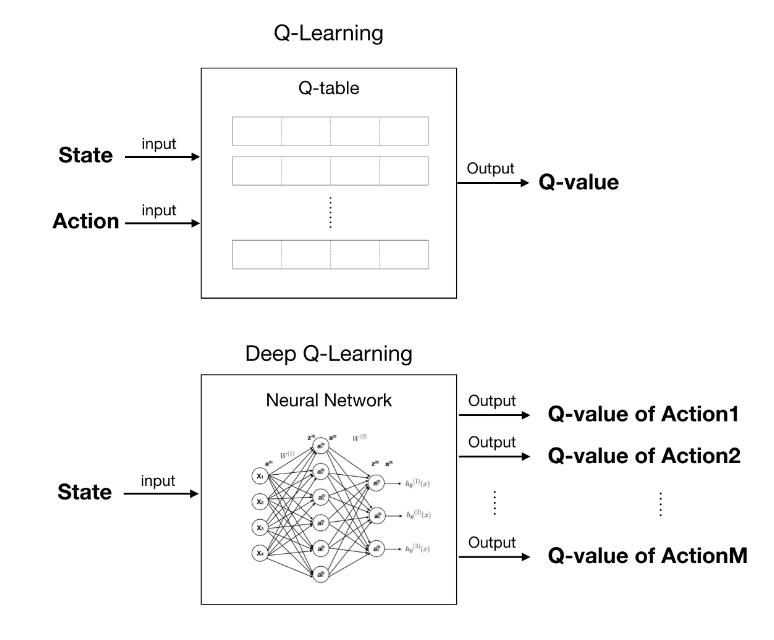
\includegraphics[width=0.5\textwidth]{Qlearning_Qnetwork.png}
\caption{Comparação entre o \emph{Q-Learning} e o \emph{Deep Q-Network}.}
\label{fig:comparacao}
\end{figure}

O principal  objetivo do aprendizado por reforço é o treinamento de um agente que interage com seu ambiente e o agente executa ações e faz a  transição entre estados. Essas ações geram em troca recompensas, que podem ser negativas, se o agente faz ações que não queremos ou positivas se está se aproximando do seu objetivo, e o objetivo do agente é maximizar essas recompensas. E dessa maneira o agente aprende a desenvolver uma política. 

O Aprendizado por Reforço possui algumas dificuldades, pois o agente só recebe recompensa quando a tarefa é bem sucedida, até atingir o seu primeiro objetivo, o agente fica explorando sem saber se está mais próximo ou não do objetivo. Para contornarmos esse problema , foi criado recompensas intermediárias para facilitar o aprendizado do agente, conhecido como \emph{reward engineering}.

Cada estado em que o agente se encontra é uma consequência direta do estado anterior e da ação escolhida. Mas, note que a ação anterior é uma consequência direta do estado anterior a ela, isso ocorre até a chegada no estado terminal. Porem pode se observar que quanto mais avançamos, mais informações o agente precisa para decidir qual a melhor ação, sendo inviável o cálculo para estados com muitos antecedentes.

Para resolvermos o problema, podemos assumir que todos os processos são Markov, ou seja, qualquer estado depende apenas do estado anterior. Pode-se notar que no processo de decisão de Markov, algumas informações estão sendo perdidas, mas é de extrema importância quando se trata do cálculo de estratégias ao longo prazo.

\subsection{Equação de \emph{Bellman}}

Faz o uso de uma técnica chamada de programação dinâmica, que é uma técnica de modelagem matemática e solução de problemas de decisão sequenciais desenvolvida por Richard Bellman. Suponha que se sabe o valor da recompensa esperada para cada ação, logo, devemos escolher as ações que gerará a maior recompensa. Essa recompensa cumulativa é denominado \emph{Q-value} e podemos escrever como
$$Q(s,a)=\gamma \max_a{Q(s',a)}$$
Essa equação nos diz que o valor Q do estado s é calculado como sendo a soma da recompensa imediata escolhendo-se a ação a com a soma do maior valor Q, e o $\gamma$ é chamado de fator de desconto, que controla a importância das recompensas de longo prazo com as de recompensas imediatas.

Essa é a chamada Equação de \emph{Bellman} e tem uma importância muito grande, pois mesmo mantendo a suposição de Markov, a natureza recursiva da Equação de \emph{Bellman} permite que as recompensas dos estados futuros se propaguem para os estados passados. E não há necessidade de saber os verdadeiros valores de Q quando é iniciado, pois por ser recursivo, sempre atualizara os valores, convergindo para os valores reais.

\subsection{\emph{Deep Q-Networks}}

Com a utilização da equação de \emph{Bellman}, temos uma estrategia, que é executar a ação que acabará acarretando na maior recompensa acumulada, isso pode ser feito em qualquer estado. Mas note que por ser um algoritmo guloso, temos um problema que é selecionar sempre as mesmas melhores ações, e nunca tentar algo novo e perder algo melhor. Para resolver esse problema, utilizamos a chamada \emph{$\varepsilon-greedy$} que consiste em escolher a \emph{greedy action} com uma probabilidade de $p=1-\varepsilon$, ou uma ação aleatória com probabilidade $p=\varepsilon$. Fornecendo assim, uma chance para o agente explorar coisas novas.

Para o \emph{Deep Q-Network} só faz sentido utilizar a Equação de \emph{Bellman} como a função de custo, e o nosso objetivo é quando o valor de Q atinge seu valor convergente, e para minimizar essa diferença faremos o uso do método dos mínimos quadrados, onde
$$Loss=[Q(s,a;\theta)-(r(s,a)+\gamma\max_a Q(s',a;\theta))]^2$$
$$MMQ = \frac{1}{n}\sum_1^n (y_i-y'_i)^2$$

\section{Implementação}

O código do projeto foi baseado na arquitetura do Laboratório 12 da disciplina CT-213- Inteligência Artificial para robótica móvel - ministrada pelo professor doutor Marcos Máximo no Instituto Tecnológico da Aeronáutica (ITA). Para executar os códigos, é preciso ter o ambiente padrão utilizado na disciplina, com a biblioteca \emph{gym} e o complemento \emph{box2d} instalados. A implementação foi feita em 4 arquivos, a saber:
\begin{itemize}
   \item dqn\underline{ }agent.py 
   \item utils.py 
   \item train\underline{ }dqn.py 
   \item evaluate\underline{ }dqn.py 
 \end{itemize}

\subsection{Agente da rede neural}
 No arquivo dqn\underline{ }agent.py está implementada o agente da rede neural profunda, bem como sua tomada de decisão e processos relacionados à atualização de sua política. Optamos por utilizar uma rede neural composta de 3 camadas densas, com funções de ativação \emph{relu} nas camadas densas e \emph{linear} na camada de saída. Como função \emph{loss}, utilizou-se a média quadrática dos erros. A fim de tentar maximizar os resultados obtidos, testamos diferentes números de neurônios nas camadas densas. Os pares números de neurônios utilizados para as camadas densas foram 64 e 64; 120 e 150; 128 e 128; 150 e 150. A Figura 3 mostra a síntese da arquitetura da rede neural implementada com 150 e 150 neurônios nas camadas densas.
\begin{figure}[H]
\centering
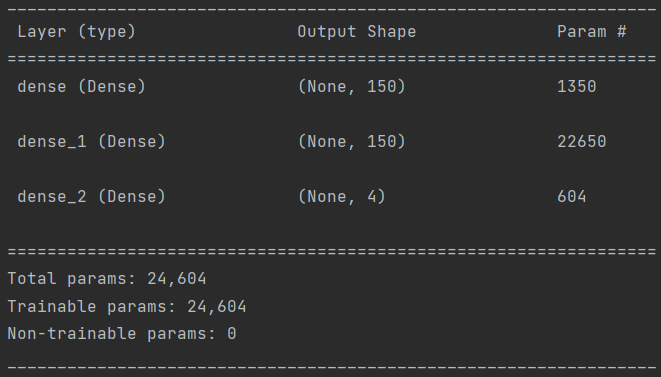
\includegraphics[width=0.5\textwidth]{rede.png}
\caption{Síntese da rede neural utilizada}
\label{fig:comparacao}
\end{figure}
Além de utilizarmos diferentes números de neurônios para treinar o agente, também realizamos os treinamentos com diferentes parâmetros a fim de tentar maximizar o seu aprendizado. A saber, utilizamos diferentes valores do parâmetro \(\epsilon\) utilizado na política \(\epsilon\)\emph{-greedy}, diferentes taxas de decaimento do \(\epsilon\) e diferentes taxas de aprendizado da rede assunto que será melhor abordado na seção V. 
 
\subsection{Úteis}
No arquivo utils.py implementamos a \emph{reward engineering} utilizada para melhorar a recompensa proposta pelo \emph{framework} do \emph{OpenAI Gym}. Foram utilizados diferentes tipos de recompensa intermediária para tentar acelerar o processo de aprendizado do agente, dentre as quais se pode citar: recompensar o agente por se aproximar da posição de pouso, diminuir os módulos de sua velocidade linear e sua velocidade angular, tocar um ou dois pés no solo, e penalizar o agente por se afastar da posição de pouso, permanecer um período longo em voo, aumentar o módulo da velocidade linear ou da velocidade angular, obter uma angulação superior a 20$^{\circ}$, possuir uma velocidade de módulo elevado em um instante de tempo superior ao equivalente a dois quintas da duração de um episódio. Ressalta-se que nem todos os métodos citados foram utilizados simultaneamente: tentamos diferentes combinações deles, a fim de tentar obter a melhor função de \emph{reward engineering} para acelerar o aprendizado do agente. Abordaremos melhor esse tema na seção V.
\subsection{Treinamento}
No arquivo train\underline{ }dqn.py está a implementação do treinamento da rede neural, que utiliza o agente proposto. Para realizar o treinamento, utilizou-se diferentes estratégias, as quais divergiam pelo número de episódios de treinamento e tamanho do \emph{batch} utilizado.  

\subsection{Avaliação}
Avalia o desempenho da rede neural treinada. Para isso, a rede neural é posta em ação por 30 episódios e, ao término de cada um, é fornecido seu tempo de duração e a recompensa recebida pelo agente. No final, o código calcula a média das recompensas recebidas. Para avaliar se um episódio foi bem sucedido ou não, desativa-se a \emph{reward engineering} implementada, a fim de manter as recompensas originais do problema. Assim, uma recompensa final superior a 200 pontos indica que o agente conseguiu concluir a tarefa com sucesso. Por fim, como o problema proposto é muito complexo, possuindo 8 dimensões de observação, não é possível representar visualmente bem a política seguida pelo agente em um mapa de duas dimensões. 

\section{Resultados e Discussões}

\subsection{Arquitetura da Rede Neural}
Dentre os pares de números de neurônios apresentados na seção \emph{IV.A}, para um mesmo número de treinamentos o par 150 e 150 apresentou melhor convergência, \emph{i.e.}, apresentou maior \emph{reward} média em função do número de episódios. Tal verificação foi feita utilizando-se diferentes métodos de \emph{reward engineering} e um número de episódios de treinamento igual a 500. 
A arquitetura escolhida para a rede neural mostra-se, por fim, em concordância com outros trabalhos que se utilizaram de uma rede neural semelhante para resolver o mesmo problema[3], embora não se verifica uma diferença muito significativa de desempenho para diferentes pares de números de neurônios[3].

\subsection{Hiperparâmetros}
Nos diversos treinamentos realizados, a taxa de aprendizagem da rede neural mais utilizada foi de 0.001. Outro valor testado, o qual não apresentou resultados mais satisfatórios foi de 0.005. Trabalhos semelhantes, apontam que a taxa de aprendizagem mais adequada é de 0.0001[4], embora ainda apresentem bons resultados nesse problema com o valor de 0.001. O parâmetro \(\gamma\) utilizado foi de 0.95 e outros valores não puderem ser testados por falta de tempo útil para a execução dos treinamentos. Uma comparação feita entre os valores de 0.9, 0.99 e 0.999 indicam o valor 0.99 como sendo o mais adequado[4]. Já o hiperparâmetro \(\epsilon\) foi ostensivamente variado, bem como sua taxa de decaimento, a fim de se buscar o melhor método de treinamento.
O valor mínimo de \(\epsilon\) utilizado, após o qual o decaimento é desativado, foi mantido constante e igual a 0.01. Uma melhor descrição dos testes feitos com o hiperparâmetro \(\epsilon\) se encontra na seção \emph{V.C}.

\subsection{Treinamento e \emph{reward engineering}}
Devido ao tempo escasso para execução do projeto e a limitações de poder computacional, optamos por realizar treinamentos com número de episódios reduzido em comparação aos treinamentos realizados em outros trabalhos[3, 4]. Assim, para testar os diferentes métodos de \emph{reward engineering} e diferentes valores dos hiperparâmetros, realizaram-se majoritariamente treinamentos de 300, 500, 800 e 900 episódios.  
Primeiramente, realizou-se um treinamento de 300 episódios com \(\epsilon\) igual a 0.5 e taxa de decaimento 0.98, sem utilização de \emph{reward engineering}. O agente não foi capaz de concluir a tarefa nem uma vez durante esse treinamento. 
Em seguida, prosseguiu-se com o teste de diferentes métodos de \emph{reward engineering}, conforme descrito na seção \emph{III}, com treinamentos de 300 episódios de duração e tamanhos de \emph{batch} variando entre 8, 16, 32, 64 e 128. Tentamos diversas políticas, inclusive políticas que penalizassem o agente depois de passado um determinado tempo do episódio - optou-se por fazê-lo pois, após determinados treinamentos, o agente adotou políticas que o faziam flutuar na mesma posição durante todo o episódio-. Chegamos a conclusão, no fim, que era interessante recompensar o agente positivamente por diminuir sua velocidade linear e sua velocidade angular, e por diminuir sua distância ao objetivo, ao mesmo tempo que se penalizam as ações contrárias a essas, conforme os pesos:
$$reward = reward + 80\cdot(vt-vt1) - 60\cdot|omegat-omegat1| + $$ $$100\cdot(dt-dt1) + pouso$$

Em que \emph{t} representa o instante t e \emph{t1} o instante t+1; \emph{v} é a velocidade linear; \emph{d} é a distância ao objetivo; \emph{omega} a velocidade angular e \emph{pouso} é uma pontuação dada por tocar os pés no solo (um deles ou ambos). 
Verificaram-se bons resultados para o valor máximo de \emph{pouso} variando entre 10 e 60. Verificaram-se bons resultados também ao se adicionar uma penalização adicional à política descrita: $-0.05\cdot|x|$, em que $x$ é a posição horizontal do agente. 

Dentre os valores de \emph{batch} testados, os que mostraram melhor desempenho foram 32 e 64 e optou-se por utilizar 32 nos treinamentos. Tais valores apresentam concordância com o que apresentam outros autores[4]. 

Uma vez definida a melhor política, realizou-se um treinamento de 4000 episódios, com valor inicial de $\epsilon$ 1.0 e taxa de decaimento 0.98. 
No entanto, como é alcançado o valor mínimo 0.01 de $\epsilon$ ao cabo de 228 episódios, nota-se que a taxa de decaimento não foi bem escolhida para o número de episódios disponível, visto que ela não é capaz de fazer suficiente exploração. O resultado foi um agente incapaz de cumprir o objetivo em mais de 10\% das tentativas. 

Em seguida, por não haver mais tempo disponível para realizar um treinamento tão longo, optou-se por tentar diferentes valores de $\epsilon$ e de taxas de decaimento. Também, a fim de tentar encontrar um balanço entre \emph{exploration} e \emph{exploitation}, decidimos por realizar três sessões de treinamento. A primeira sessão foi de 200 episódios, a segunda de 300 episódios e na terceira sessão foram testados diferentes números de episódios com diferentes valores de $\epsilon$. As Figuras 4, 5 e 6 mostram a evolução de um dos treinamentos realizados. 
\begin{figure}[H]
\centering
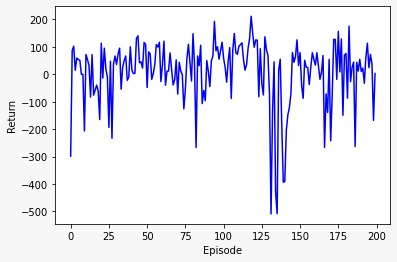
\includegraphics[width=0.5\textwidth]{t1.jpeg}
\caption{Primeira sessão de treinamento: 200 episódios.}
\label{fig:comparacao}
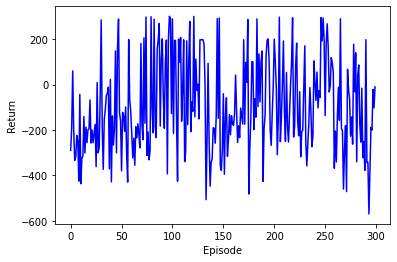
\includegraphics[width=0.5\textwidth]{t2.png}
\caption{Segunda sessão de treinamento: 300 episódios.}
\label{fig:comparacao}
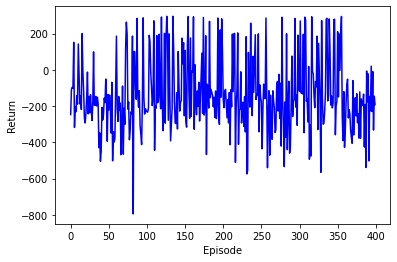
\includegraphics[width=0.5\textwidth]{t3.png}
\caption{Terceira sessão de treinamento: 300 episódios.}
\label{fig:comparacao}
\end{figure}

Devido à grande flutuação dos valores de \emph{reward}, conforme se observa nas figuras 4, 5 e 6, pode-se observar claramente que não houve convergência para uma política consistente, capaz de pousar com sucesso em mais de 70\% dos casos. Dessa forma, tentamos realizar mais treinamentos a fim de se obter uma política mais sólida. Uma das tentativas foi truncar o valor de $\epsilon$ em 0.05, cujo gráfico de recompensa durante o treinamento é apresentado na Figura 8.

\begin{figure}[H]
\centering
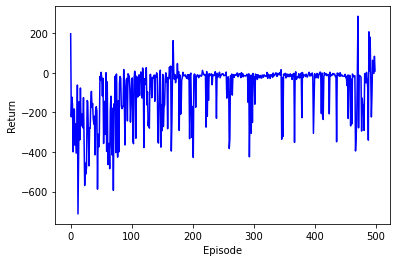
\includegraphics[width=0.5\textwidth]{outrotreino.png}
\caption{Terceira sessão de treinamento: 500 episódios com $\epsilon=0.05$ constante.}
\label{fig:comparacao}
\end{figure}

Em resumo, muitos treinamentos foram realizados, com diversas sessões, número de episódios variando entre 300 e 800, $\epsilon$ variando entre 1.0 e 0.05 - a depender se um determinado conjunto de pesos já havia passado por alguma sessão de treinamento-, taxas de decaimento variando entre 0.95 e 0.999, no entanto, nenhum foi capaz de deixar o agente com uma política robusta e consistente. Acreditamos que isso se deve ao fato de os treinamentos terem poucos episódios, com um decaimento do $\epsilon$ relativamente alto. Assim, a rede não foi capaz de adquirir experiência suficiente para o grande número de estados possível, o que se reflete na inconsistência do agente. 

 
\section{Conclusão}

Dado a intensiva e longa busca por métodos de treinamento do agente com poucos episódios (menos de 1000 episódios) sem sucesso, conclui-se que ela não pode ser realizada com a rede neural, o método de \emph{reward engineering} e os hiperparâmetros adotados neste trabalho. O melhor agente obtido com os curtos treinamentos realizados obtém sucesso na tarefa em menos de 30\% dos casos. A Figura 8 mostra o desempenho de um dos melhores agentes treinados. 

\begin{figure}[H]
\centering
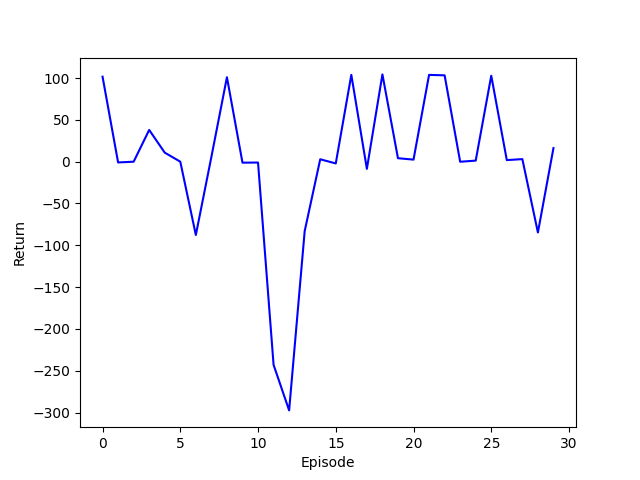
\includegraphics[width=0.5\textwidth]{dqn_evaluation.png}
\caption{Desempenho de um dos agentes treinados.}
\label{fig:comparacao}
\end{figure}

Como se pode observar, o agente se mostra extremamente inconstante, o que se deve ao curto número de episódios de treinamento realizados. Um fator a ser considerado, a fim de se obter um agente com uma política mais constante, é a troca da DQN por uma Double-DQN[4, 5]: a instabilidade pode ser causada pela atualização dos pesos enquanto a mesma rede é utilizada para avaliar as ações. Assim, o uso de duas redes (DDQN) pode ser útil para contornar esse problema[5].
Por fim, obter-se-iam melhores resultados em comparação aos aqui apresentados ao se utilizar um grande número de episódios de treinamento - pelo menos 5000 -, com uma taxa de decaimento suficientemente pequena para garantir que o agente faça a exploração necessária para a obtenção de uma política sólida com alta taxa de sucesso. 

%%%%%%%%%%%%%%%%%%%%%%%%%%%%%%%%%%%%%%%%%%%%%%%%%%%%%%%%%%%%%%%%%%%%%%%%%%%%%%%%



%%%%%%%%%%%%%%%%%%%%%%%%%%%%%%%%%%%%%%%%%%%%%%%%%%%%%%%%%%%%%%%%%%%%%%%%%%%%%%%%



%%%%%%%%%%%%%%%%%%%%%%%%%%%%%%%%%%%%%%%%%%%%%%%%%%%%%%%%%%%%%%%%%%%%%%%%%%%%%%%% 


%%%%%%%%%%%%%%%%%%%%%%%%%%%%%%%%%%%%%%%%%%%%%%%%%%%%%%%%%%%%%%%%%%%%%%%%%%%%%%%%




\begin{thebibliography}{99}

\bibitem{c1} Schraudolph, Nicol N.; Terrence, Peter Dayan; Sejnowski, J., Temporal Difference Learning of Position Evaluation in the Game of Go
\bibitem{c2} Silver, D., Schrittwieser, J., Simonyan, K. et al. Mastering the game of Go without human knowledge. Nature 550, 354–359 (2017)

\bibitem{3} Gadgil, Soham, Yunfeng Xin, and Chengzhe Xu. "Solving the lunar lander problem under uncertainty using reinforcement learning." 2020 SoutheastCon. Vol. 2. IEEE, 2020.

\bibitem{4} OpenAI Gym's LunarLander-v2 Implementation. Disponível em
<https://github.com/svpino/lunar-lander>. Acesso em 17/07/2020.

\bibitem{5}T. Lillicrap, J. Hunt, A. Pritzel, N. Heess, T. Erez, Y. Tassa, D. Silver, and D. Wierstra. Continuous Control With Deep Reinforcement Learning. (2015). arXiv preprint arXiv:1509.02971


\end{thebibliography}




\end{document}
